\documentclass[11pt]{article} % use larger type; default would be 10pt
\usepackage{amsmath}
\usepackage[x11names]{xcolor}                     %Additional colors
\usepackage{tikz}
                               %Nicer numbers

%Note about the colors: 
%  The color of the "ray" lines should not be
%  black or gray as on some printers, significant
%  aliasing distorsion becomes visible.

\begin{document}
\thispagestyle{empty} %Please, no page numbers or similar

\begin{center}
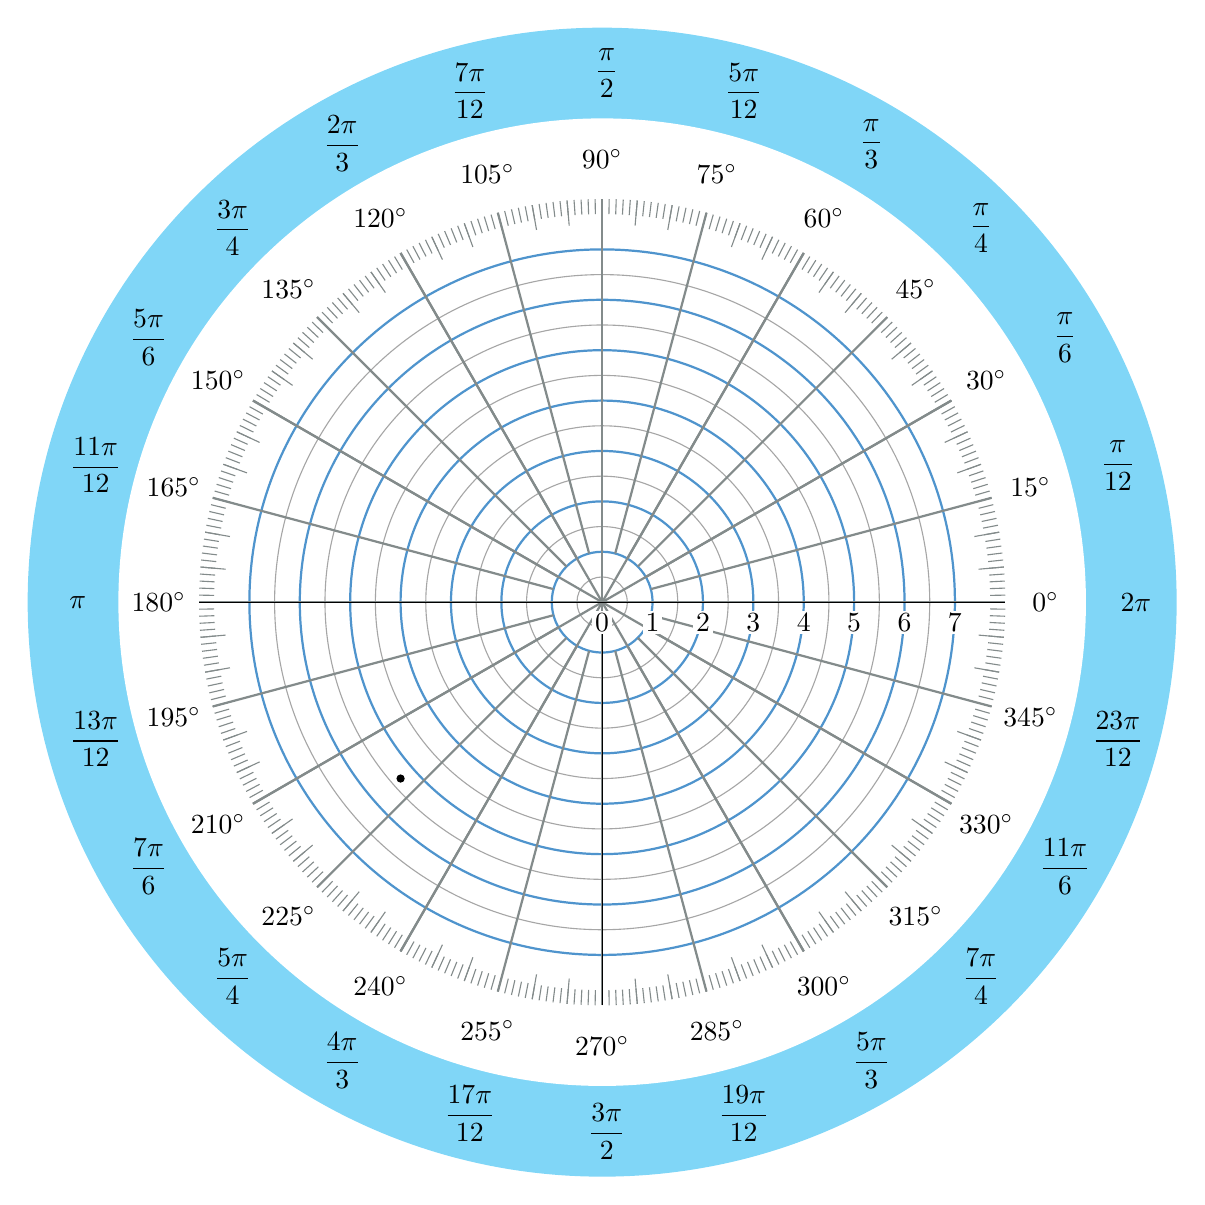
\begin{tikzpicture}[scale=0.64]
\fill[cyan!50] circle (11.4);
\fill[white] circle (9.6);
%Circles 
\foreach \r in {1, 2,...,7}
\draw[SteelBlue3, thick] (0,0) circle (\r);    
\foreach \r in {0.5, 1.5,...,7}
\draw[gray!70, thin] (0,0) circle (\r);
%1° Rays
\foreach \a in {0, 1,...,359}
\draw[Azure4] (\a:7.7) -- (\a:8);
%5° Rays
\foreach \a in {0, 5,...,359}
\draw[Azure4] (\a:7.5) -- (\a:8);      
%15° Rays
\foreach \a in {0, 15,...,359}
\draw[thick,Azure4] (\a:1) -- (\a:8); 
%30° Rays
\foreach \a in {0, 30,...,359}
\draw[thick,Azure4] (0, 0) -- (\a:8);
%Main rays
\draw (-8,0) -- (8,0);
\draw (0,-8) -- (0,-0.5);
%Angle labels  
\foreach \a in {0, 15,...,359}
\draw (\a: 8.8) node[fill=white,inner sep=.2mm] {$\a^\circ$};
%Central point
\draw[fill=black] (-4,-3.5) circle(0.7mm);
%Radius labels (background filled white)
\foreach \r in {0,1,...,7}
\draw (\r,0) node[inner sep=1pt,below=3pt,rectangle,fill=white] {$\r$};
%\draw circle (8.2);
\foreach \gwnia/\xtext in {
15/\dfrac{\pi}{12},
30/\dfrac{\pi}{6},
45/\dfrac{\pi}{4},
60/\dfrac{\pi}{3},
75/\dfrac{5\pi}{12},
90/\dfrac{\pi}{2},
105/\dfrac{7\pi}{12},
120/\dfrac{2\pi}{3},
135/\dfrac{3\pi}{4},
150/\dfrac{5\pi}{6},
165/\dfrac{11\pi}{12},
180/\pi,
195/\dfrac{13\pi}{12},
210/\dfrac{7\pi}{6},
225/\dfrac{5\pi}{4},
240/\dfrac{4\pi}{3},
255/\dfrac{17\pi}{12},
270/\dfrac{3\pi}{2},
285/\dfrac{19\pi}{12},
300/\dfrac{5\pi}{3},
315/\dfrac{7\pi}{4},
330/\dfrac{11\pi}{6},
345/\dfrac{23\pi}{12},
360/2\pi}
{\draw (\gwnia:10.5) node {{ $\xtext$}};}
\end{tikzpicture}
\end{center}

\end{document}